%%%%%%%%%%%%%%%%%%%%%%%%%%% Figure 3 Godafoss %%%%%%%%%%%%%%%%%%%%%%%%%%%%%%%
\begin{figure}[t]
 \begin{center}
  \begin{pspicture}(0,0)(15,12)
% Include graphs
   \rput[br](7.4,6){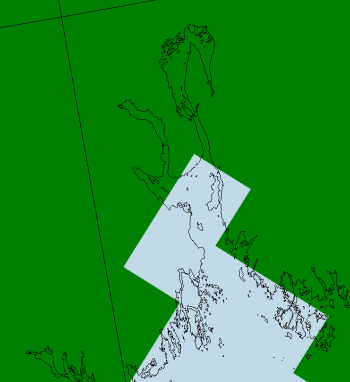
\includegraphics[height=6cm]{Oslofjord_A20_grid}}
   \rput[bl](7.5,6){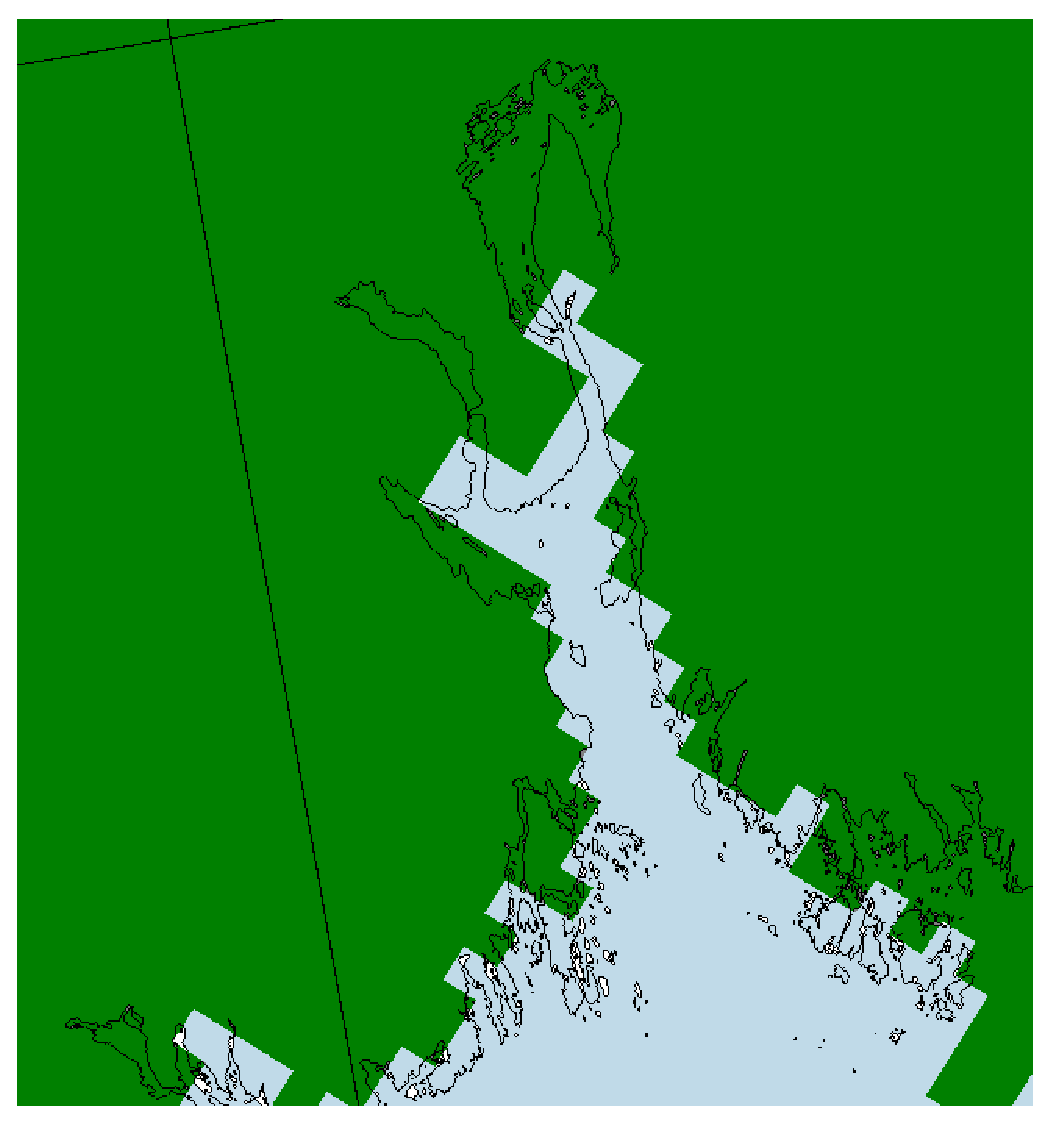
\includegraphics[height=6cm]{Oslofjord_N4_grid}}
   \rput[b](7.5,-0.2){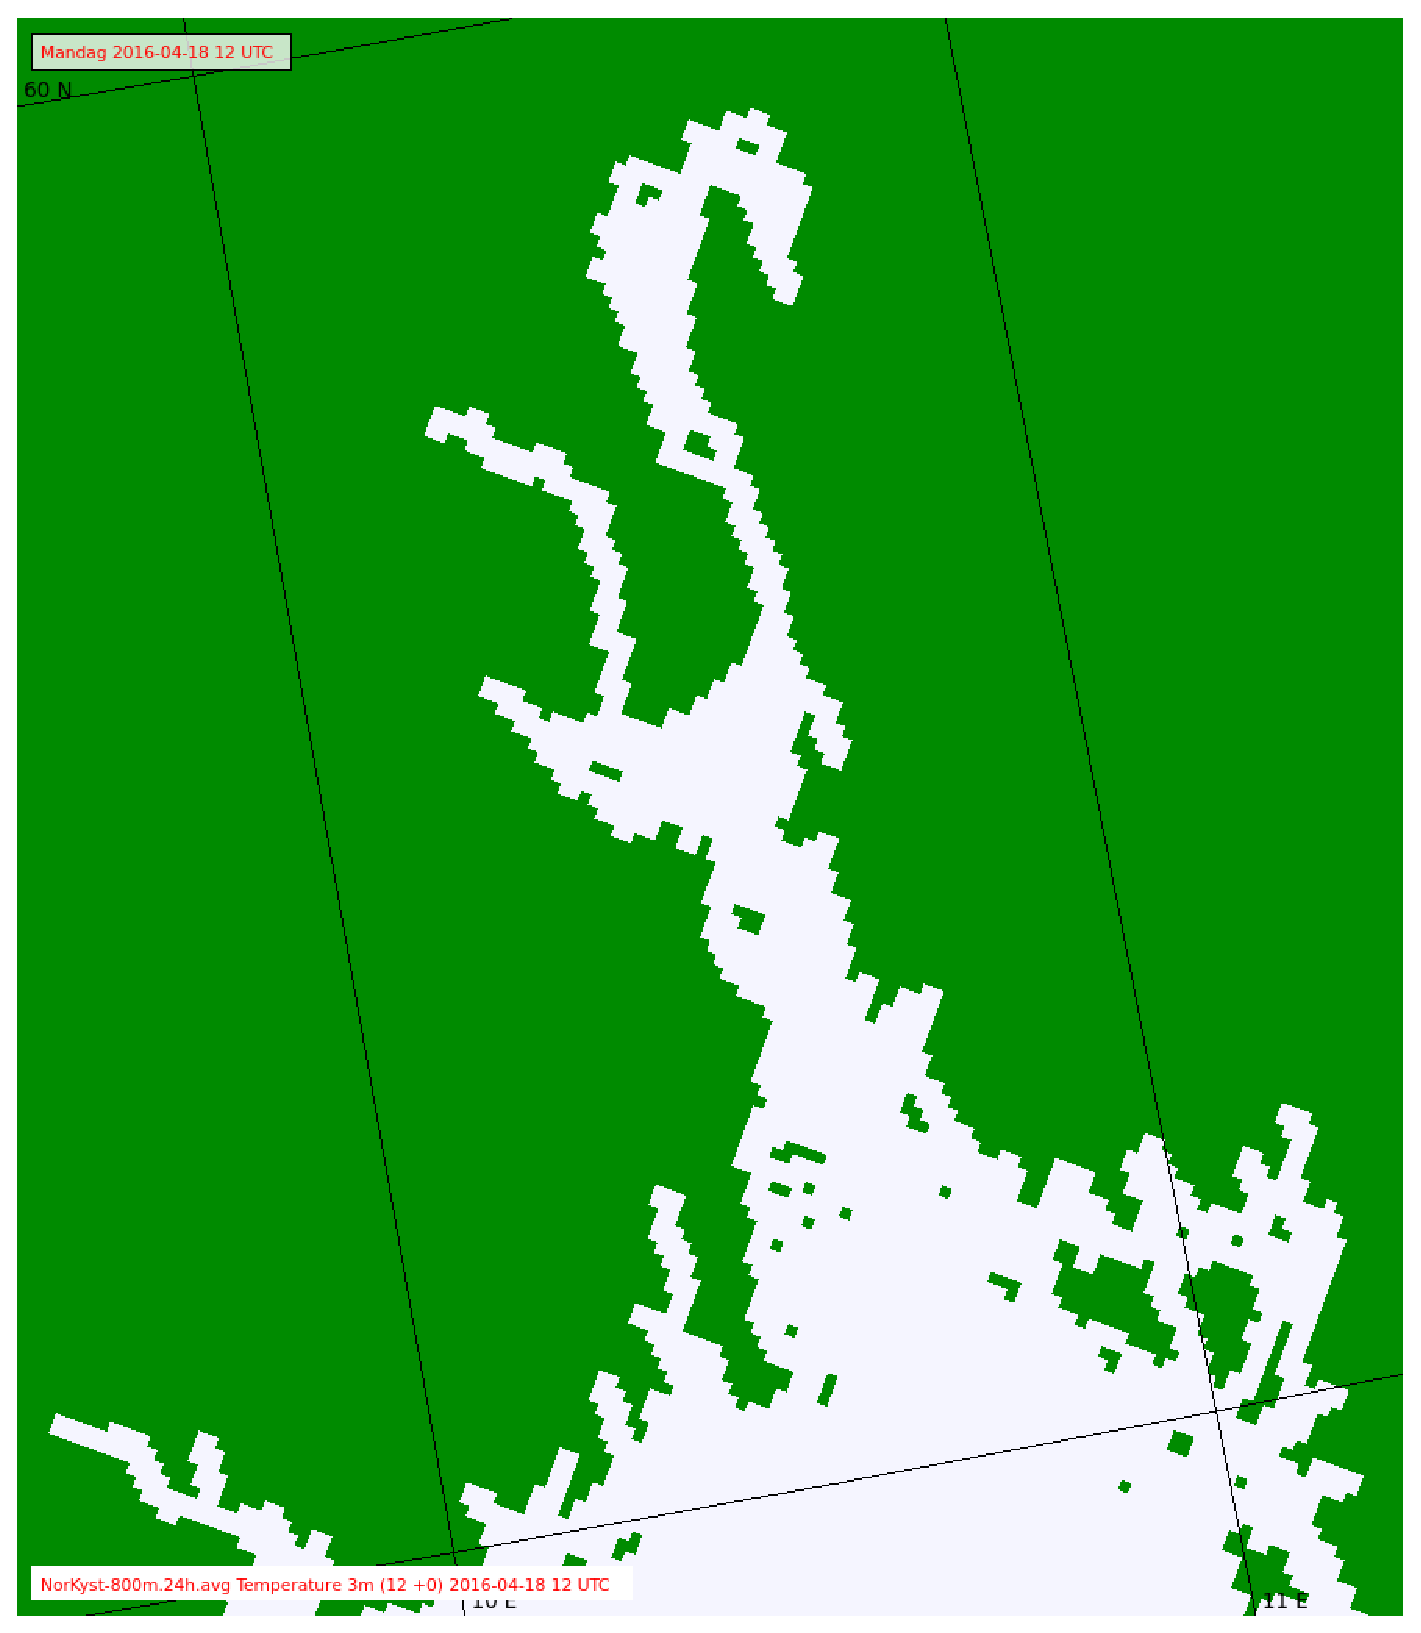
\includegraphics[height=6cm]{Oslofjord_N800_grid}}
%   \rput[bl](7.5,0.0){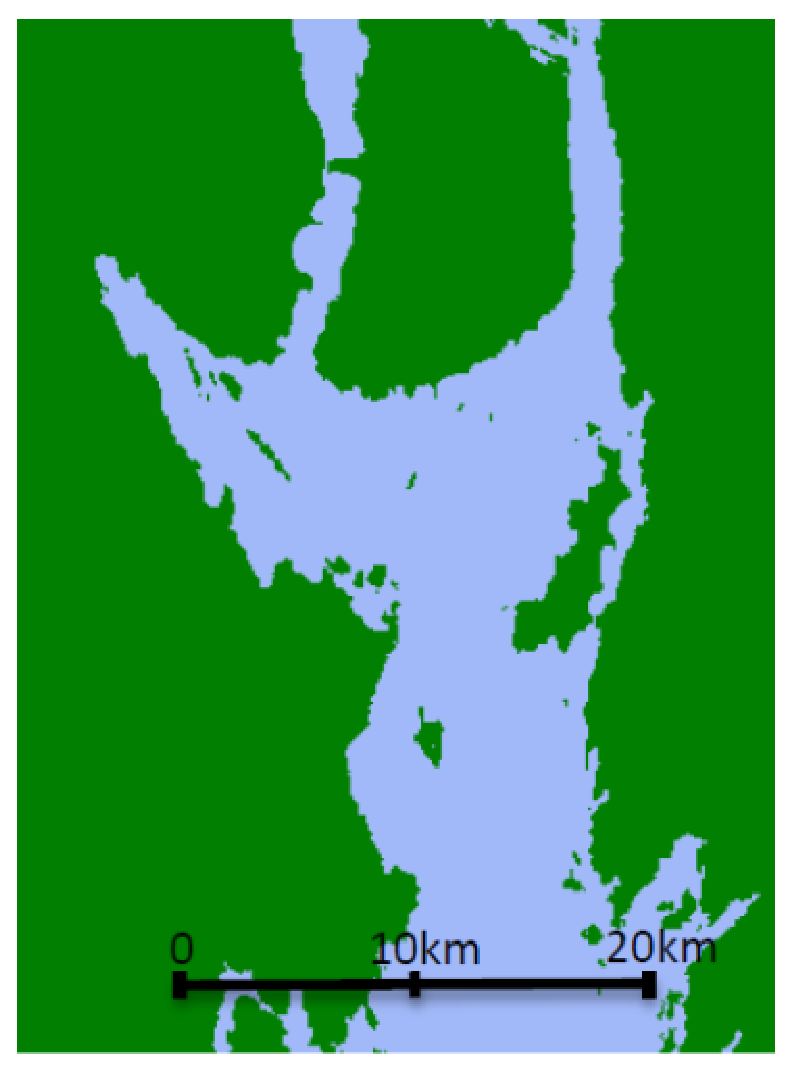
\includegraphics[height=5.2cm]{Midfjord_100m_grid}}
  \end{pspicture}
  \caption{\small Illustrated is the impact of grid resolution on how the Oslofjord is portrayed. Upper two panels show what the fjord looks like utilizing respectively a 20 km grid (left) and 4 km grid (right). Bottom panel show the same for utilizing a 800 m grid to represen the fjord. As revealed the smaller the grid size (higher grid resolution) the better the coastline geometry is represented. } 
  \label{fig:resolution}
 \end{center}
\end{figure}

